\documentclass{article}%
\usepackage[T1]{fontenc}%
\usepackage[utf8]{inputenc}%
\usepackage{lmodern}%
\usepackage{textcomp}%
\usepackage{lastpage}%
\usepackage[head=40pt,margin=0.5in,bottom=0.6in]{geometry}%
\usepackage{graphicx}%
%
\title{\textbf{Londres insiste en el diálogo del Brexit seguirá pese a pesimismo UE}}%
\author{AP}%
\date{07/03/2019}%
%
\begin{document}%
\normalsize%
\maketitle%
\textbf{URL: }%
http://www.eluniversal.com/internacional/34995/londres{-}insiste{-}en{-}el{-}dialogo{-}del{-}brexit{-}seguira{-}pese{-}a{-}pesimismo{-}ue\newline%
%
\textbf{Periodico: }%
EU, %
ID: %
34995, %
Seccion: %
internacional\newline%
%
\textbf{Palabras Claves: }%
NO\_TIENE\newline%
%
\textbf{Derecho: }%
2.1%
, Otros Derechos: %
\newline%
%
\textbf{\textit{La Unión Europea afirmó por su parte que las “difíciles” conversaciones no han logrado avances porque las propuestas británicas no son realistas}}%
\newline%
\newline%
%
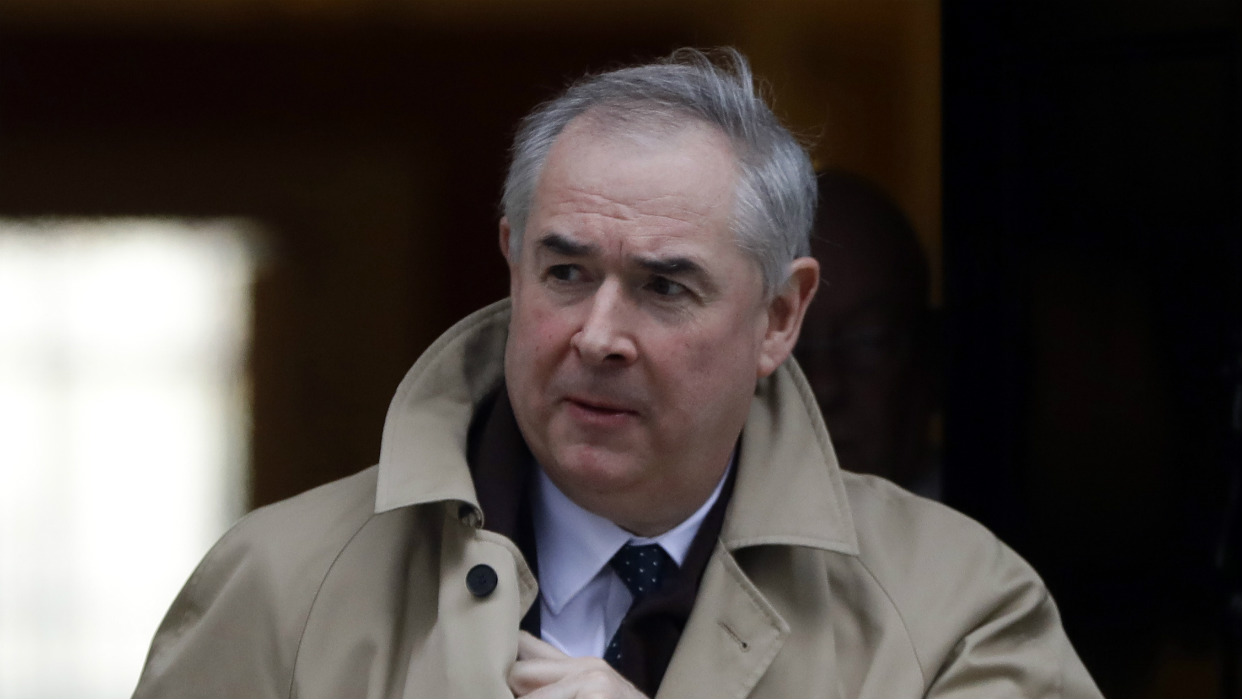
\includegraphics[width=300px]{EU_34995.jpg}%
\newline%
%
Londres.{-} Las negociaciones con la Unión Europea (UE) para el Brexit continuarán durante el fin de semana, mientras el Reino Unido intenta lograr cambios en su acuerdo de divorcio con Bruselas antes de una votación parlamentaria la próxima semana, dijo el fiscal general británico.%
\newline%
%
La UE afirmó por su parte que las “difíciles” conversaciones no han logrado avances porque las propuestas británicas no son realistas, indicó AP.%
\newline%
%
Pero el fiscal general, Geoffrey Cox, señaló el jueves que las "discusiones centradas, detalladas y cuidadosas” se reanudarán “en breve”.%
\newline%
%
Está previsto que el Reino Unido abandone el bloque el próximo 29 de marzo, pero su parlamento rechazó el acuerdo de salida forjado entre Londres y Bruselas.%
\newline%
%
La primera ministra Theresa May está tratando de conseguir modificaciones, pero la UE insiste en que no reabrirá el documento, que es legalmente vinculante.%
\newline%
%
La Cámara de los Comunes votará de nuevo el pacto el martes. Si sale rechazado, los legisladores podrían intentar demorar el Brexit.%
\newline%
%
\end{document}